\documentclass[11pt,conference]{IEEEtran}
\IEEEoverridecommandlockouts
\usepackage{cite}
\usepackage{amsmath,amssymb,amsfonts}
\usepackage{algorithmic}
\usepackage{graphicx}
\usepackage{hyperref}
\usepackage{textcomp}
\usepackage{xcolor}
\def\BibTeX{{\rm B\kern-.05em{\sc i\kern-.025em b}\kern-.08em
    T\kern-.1667em\lower.7ex\hbox{E}\kern-.125emX}}
\begin{document}

\title{Two-Phase Commit Using Blockchain}

\author{\IEEEauthorblockN{Benjamin Marks}
\IEEEauthorblockA{\textit{Stanford University} \\
benmarks@stanford.edu}
\and
\IEEEauthorblockN{Heron Yang}
\IEEEauthorblockA{\textit{Stanford University} \\
heronyang@stanford.edu}
\and
\IEEEauthorblockN{Yuewei Na}
\IEEEauthorblockA{\textit{Stanford University} \\
yueweina@stanford.edu}
}

\maketitle

\begin{abstract}
We created a decentralized system that uses a public blockchain as a two-phase commit (2PC) coordinator, so users can securely commit an atomic transaction across any databases that support our interface. Users treat our system as one large database with ACID, despite being composed of many individual databases that are unaware of each other’s existence. By using a blockchain as a coordinator, it is resilient to failures such as network outages, power outages, and disk failures that cause traditional 2PC implementations to block. Our initial integration is with the Ethereum blockchain and LMDB databases; however, our system provides a generic interface to integrate with other blockchains and databases.
\end{abstract}

\begin{IEEEkeywords}
atomic commit, blockchain, smart contract, distributed system, database transaction
\end{IEEEkeywords}

\section{Introduction}
Two-Phase Commit (2PC) is a widely-adopted protocol that allows distributed systems to reach the consensus of distributed transactions. It ensures that the transaction can be either committed or aborted at all distributed machines. However, blocking is proven [3] to be to be inevitable even in
synchronous systems where bounds on delays can be reliably estimated. 

Since the invention of Bitcoin, the underlying technology, the blockchain, not only gained attraction from  cryptocurrency systems like Ethereum but also academic research about computer systems. At its core, blockchain is a protocol of reaching consensus by using Proof-of-Work or Proof-of-Stake [//TODO: reference goes here]. Previous work [1] has shown that synchronous blockchain can increase the reliability of the original 2PC protocol and also make it non-blocking when various kinds of failures happen.

In this paper, we further extended the previous work with an optimized system architecture and properly designed interfaces. These contributions make 2PC with blockchain work in production and at scale. Compared to the traditional version of 2PC protocol [2], our proposed approach increases extensibility, scalability and reliability.


\subsubsection{Extensibility}
We can plug any blockchain, regardless of whether it is public/permissionless or private/permissioned, into our blockchain interface which exposes \texttt{StartVoting()}, \texttt{Vote()}, \texttt{GetVotingDecision()}. We can also plug any database system that has ACID support into our transaction delegation interface, which implements common transaction operations - \texttt{Begin()}, \texttt{Commit()}, \texttt{Abort()}, \texttt{Get()}, \texttt{Put()}.

\subsubsection{Scalability}
We design our coordinator  to be light-weight to handle high throughput and horizontally scalable. This is achieved by delegating coordination and voting work to the blockchain. The delegation makes the coordinator stateless and allows many coordinator jobs to co-exist to balance the load and tolerate job failures. Adding a cohort to the system is as simple as making potential clients aware of the address of the newly added cohort, so our system is horizontally scalable.

\subsubsection{Reliability}
Our system has better reliability than the traditional 2PC protocol for two reasons. First, the system leverages blockchain to maintain the coordination state. The stateless coordinator can easily recover as long as it knows the participating cohorts. Second, The coordinator is stateless and horizontally scalable. We can keep multiple jobs running concurrently and place a load-balancing layer on top of it. 

\section{Design Overview}
\subsection{Architecture and Components} \label{components}
We define a transaction as a list of operations starting with \texttt{BEGIN} followed by multiple \texttt{GET} or \texttt{PUT} and ending with \texttt{COMMIT}. The client creates a transaction and requests the coordinator to commit. The coordinator distributes the transaction to the corresponding cohorts to prepare and then offloads the remaining 2PC responsibility to the blockchain. Each cohort prepares the transaction locally, votes to the blockchain if ready, checks on Blockchain to see if a transaction should be committed, then finally commits the transaction to its database.

The architecture is similar to the traditional 2PC architecture where we have one coordinator and multiple cohorts - except each cohort talks to the blockchain directly to vote and to look up the voting decision as the coordinator offload the 2PC voting responsibility to the blockchain.

We describe details of each component and each in the remaining \ref{components}, the complete flow of handling a successful transaction in \ref{txnflow}, and how we handle failures in \ref{failurecases}.
\begin{figure}[h]
\centering
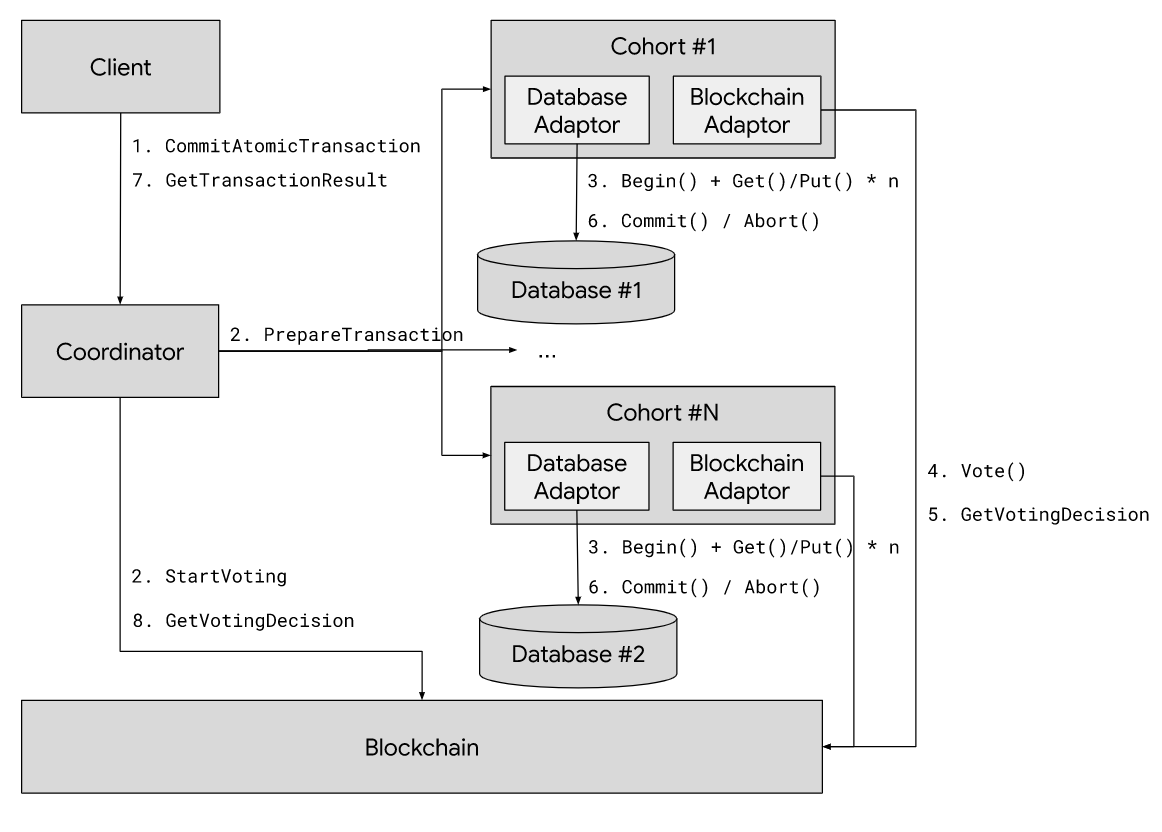
\includegraphics[width=0.4\textwidth]{./diagram.png}
\caption{Fig 1. This diagram displays the main components within the whole architecture and example steps of successfully committing a transaction.}
\label{fig:Panel}
\end{figure}

\subsubsection{Blockchain} \label{blockchain}
The blockchain component performs a 2PC protocol, so it’s responsible for tracking voting states of each transaction and making decisions of committing. The implementation uses Ethereum smart contracts to store the followings states of each transaction (indexed by the transaction ID) internally:
$transaction\_state$ stores voting states of each cohort of a transaction.
$transaction\_config$ stores the transaction configure of each transaction including the number of cohorts and the vote timeout time.

We designed a \texttt{\\BlockchainAdapter} interface, which exposes the following APIs externally to the coordinator and the cohort:
\texttt{StartVoting(\\transaction\_id, cohorts, vote\_timeout\_time)} Called by the coordinator to start voting on a transaction. $cohorts$ is the number of cohorts that will vote on this transaction later. $vote\_timeout\_time$ is the absolute time on the blockchain when the 2PC stops taking votes.
\texttt{Vote(transaction\_id, cohort\_id, ballot)} Called by the cohort to vote $COMMIT$ or $ABORT$ on a transaction before timeout.
\texttt{GetVotingDecision(transaction\_id)} Called by any component to check the voting state on a transaction.

\texttt{StartVoting} initializes the states for a transaction and \texttt{Vote} updates the voting status of a transaction. \texttt{GetVotingDecision} makes the decision by following the below logic:
If any $ABORT$ vote is received, return an $ABORT$ decision.
If all $COMMIT$ votes are received, return a $COMMIT$ decision.
If not (1) and not (2), return an $ABORT$ decision if timed out; otherwise, return a $PENDING$ decision.

\subsubsection{Database} \label{database}
The database component is responsible for committing sub-transactions in each cohort and abstracts typical ACID databases with 5 APIs in a DatabaseAdapter:
\begin{itemize}
  \item \texttt{Begin()}:  starts a transaction
  \item \texttt{Commit()}: commits a started transaction
  \item \texttt{Abort()}: aborts a started transaction
  \item \texttt{Put(key, value)}: puts value in a row whose primary key is key 
  \item \texttt{Get(key)}: gets the value from the row whose primary key is key 
\end{itemize}






We require the underlying database to be ACID because the database can handle locks and transactions natively without requiring cohorts to implement complicated locking logic for Put and Get operations. However, for databases that only support weak snapshot isolation (e.g. LMDB [4]), the cohort needs a single write lock to prevent other write transactions to be started to make sure that transactions are serialized. 

\subsubsection{Coordinator} \label{coordinator}
The coordinator exposes two APIs to the clients:
\begin{itemize}
  \item \texttt{CommitAtomicTransaction(
    CommitAtomicTransactionRequest, CommitAtomicTransactionResponse)}
  \item \texttt{GetTransactionResult(
    GetTransactionResultRequest, GetTransactionResultResponse)}
\end{itemize}   

The data key space is split into $namespaces$, each of which corresponds to the single cohort responsible for all keys in that range.  When the coordinator receives a \texttt{\\CommitAtomicTransaction} call from the client, it first sends \texttt{StartVoting} to the blockchain to trace the voting status from the cohorts. Then it decomposes the transaction into sub-transactions, which will be executed in the cohorts, based on the $namespace$ of each operation. After transaction decomposition, the coordinator sends \texttt{PrepareTransaction} requests with the sub-transactions to the cohorts. Different from the traditional 2PC protocol, we design our coordinator to delegate voting and coordination work to the blockchain. From here on, the coordinator no longer handles any work unless \texttt{GetTransactionResult} is requested from the client.

When the client sends \texttt{GetTransactionResult} to the coordinator, the coordinator reads the transaction status from the blockchain. If the blockchain returns a PENDING or ABORTED status, the coordinator will return the status directly. If the transaction is COMMITTED, the coordinator will send requests to the cohorts to fetch the Get results and then return the status with the Get results. If not all cohorts return the Get results (e.g. due to crashes or network latency), the coordinator will send a partial response to the client with the ones that responded along with an indicator that the response is not yet complete.

As described in the handling failures section, the coordinator does not need to persist any information to disk as all voting information is stored in the blockchain and all other information is also known by the client.

\subsubsection{Cohort} \label{cohort}

The cohort exposes two APIs to the coordinator:
\begin{itemize}
  \item \texttt{PrepareTransaction(
    PrepareTransactionRequest, PrepareTransactionResponse)}
  \item \texttt{GetTransactionResult(
    GetTransactionResultRequest, GetTransactionResultResponse)}
\end{itemize} 

The $PrepareTransactionRequest$ contains a $transaction\_id$, a list of operations of the sub-transaction and a vote timeout time, after which the blockchain will not accept votes. When a cohort receives a \texttt{PrepareTransaction} request from the coordinator, it takes these steps: 
\begin{enumerate}
  \item Start a new thread in the thread pool.
  \item Create a \texttt{DatabaseAdapter} object.
  \item Start a transaction with 
  \texttt{DatabaseAdapter\\::Begin()}. 
  \item Acquire the relevant locks for the sub-transaction. 
  \item Execute a series of requested Put or Get operations in the sub-transaction. 
If any operation is reported invalid by the database or locks cannot be acquired in time, the cohort will send an $ABORT$ ballot to the blockchain via \texttt{BlockchainAdapter::Vote()}.
  \item If all operations succeed, it will store the retrieved Get values in an in-memory hashmap as well as persistently on disk keyed by the $transaction\_id$ to prepare for future \texttt{GetTransactionResult} calls.
  \item Set a timer based on the vote timeout time.
  \item If the timer reaches the vote timeout time, it will send a request \texttt{BlockchainAdapter::\\GetVotingDecision(transaction\_id)} to the blockchain. 
  \begin{enumerate}
    \item If the blockchain states that the transaction should be committed, it will call \texttt{DatabaseAdapter::Commit()}.
    \item If the blockchain states that the transaction should be aborted, it will call \texttt{DatabaseAdapter::Abort()}.
  \end{enumerate}
  
\end{enumerate}



When the cohort receives a \texttt{GetTransaction\-Result} request and has committed the transaction, it simply reads the in-memory hashmap based on the $transaction\_id$ in the request and returns the got values as response. If it has not yet received a commit or abort response from the blockchain, it returns a pending response instead.

\subsection{System Interactions (a.k.a Life of a Transaction)} \label{txnflow}
This section describes the end-to-end life of a transaction without handling failures.

\begin{enumerate}
\item The client composes a transaction request and passes it to the coordinator through \texttt{\\CommitAomticTransaction}. The coordinator returns a transaction ID for the client to look up the transaction result later.
\item The coordinator asks the blockchain to trace votes for the new transaction through \texttt{StartVoting}.
\item The coordinator decomposes the transaction into sub-transactions and distributes them to the corresponding cohort through \texttt{PrepareTransaction}.
\item Each cohort executes a sub-transaction by acquiring locks and forwarding the operations to the database up to the point before Commit(). The cohort writes an entry to the redo log to recover in case it crashes. Additionally, the cohort writes the \texttt{GET} operation results to disk for faster responses after a crash and recovery.
\item The cohort votes to the blockchain through \texttt{Vote} indicating that it wants to commit or abort the transaction.
\item The cohort waits until the expected transaction timeout time and gets the voting decision from the blockchain through \texttt{GetVotingDecision}.
\item If the voting decision is to commit the transaction, cohort commits the sub-transaction onto the database and releases any acquired locks; otherwise, it aborts the sub-transaction in the database and releases any acquired locks.
\item (Independent of the previous steps) The client waits until the timeout time and requests the transaction result from the coordinator through \texttt{GetTransactionResult}, using the transaction ID given in step 1.
\item The coordinator gets (1) the voting decision of the inquiry transaction from the blockchain through \texttt{GetTransactionResult} and (2) the GET operation results from each cohort.
\end{enumerate}

\subsection{Handling Failures} \label{failurecases}
As described above, one of the main benefits of our system compared to traditional 2PC implementations is improved resiliency. By delegating the voting and coordination to the blockchain, our system does not block on any one machine that crashes or has a partitioned network.

\subsubsection{Crash of the coordinator}
The state of the coordinator includes only the list of which cohorts are involved in each active transaction. Thus if the coordinator crashes, when it recovers, it will respond to client requests for the \texttt{GET} responses of the transaction by indicating that it is unable to find the transaction. As a result, the client can directly ask the cohorts what the \texttt{GET} responses of the transaction are. Unlike in traditional 2PC, where the coordinator stores how each cohort has voted, in our design, this information is stored in the blockchain. Our system is resilient to such crashes, as the transaction does not need to block on the coordinator’s recovery.

\subsubsection{Crash of a cohort}
Our system is also resilient to crashes of cohorts, as these crashes do not cause any other cohorts to block for longer than the vote timeout time.  If a cohort crashes before sending a vote to commit, then the blockchain will wait until the vote timeout time and all cohorts will abort the transaction. If a cohort crashes after voting to commit and the blockchain decides that the transaction should commit, then the cohort will replay all transactions that committed while it crashed and recovered. To replay the transactions, the cohort will acquire the same locks it had for the transactions and send the relevant Put and Get requests to the database and commit the transactions in the database. Since it has already computed the response, if the coordinator asks for the get responses for any of these transactions, the cohort can safely return them, even if they have not yet committed in the database. This can be implemented in the future, but we decided not to include it in our first version. 

\subsubsection{Slow blockchain}
We use Ethereum for our blockchain implementation. According to [this article], it takes around 15 seconds to 5 minutes to process a blockchain transaction on Ethereum, which indicates that the blockchain is relatively slow compared to other components within our system. A slow blockchain affects the number of commit votes to collect before the vote timeout time, which leads to more transactions to abort eventually; however, the blockchain slowness doesn’t affect the promised atomicity. The client or the coordinator can specify a longer timeout time if needed.


\section{Implementation}
In this section we first describe the implementation of our overall system. Then, we illustrate the implementation of individual components.

\subsection{Environment}
We implemented the coordinator and the cohorts with about 2800 lines of C++ code. For communications between components, we used gPRC and ProtoBuf. For providing the extensibility of swapping different database and blockchain implementations, we provided generic interfaces. We tested end-to-end behavior on a single machine with different processes simulating each component.

\subsubsection{Blockchain}
We wrote our two-phase-commit smart contract with Solidity and developed it with Truffle [\url{https://trufflesuite.com/}]. Truffle provides the development environment for us to compile smart contracts, test it, and deploy it locally for debugging. Once we’ve deployed our smart contract, the coordinator and the cohorts can interact with the contract through a smart contract client library. However, we didn’t find a proper C++ smart contract client library to use, so we use a JavaScript library (web.js[\url{https://web3js.readthedocs.io/en/v1.7.3/}]) instead and add an additional gRPC layer to translate to C++.

While testing in the Truffle development, we learned the gas used for successfully committing a transaction with two cohorts is around 0.33 USD [\href{https://automatedwebtools.com/gwei-to-usd-calculator/}{reference}] (see \ref{appendix} for breakdowns).

\subsubsection{Database}
We designed the DatabaseAdapter interface and implemented the methods with LMDB primitives. LMDB provides process-oriented functions like \texttt{Open()}, \texttt{Begin()}, \texttt{Commit()}, \texttt{Put()}, \texttt{Get()}. Our object-oriented C++ implementation has almost 500 lines of code. We chose LMDB because it is fast, lightweight and easy to test in memory; however, the interface is also extensible to other databases like SQLite [6].

\subsubsection{Coordinator}
The coordinator deterministically computes a global identifier for the transaction based on the client’s provided identifier and the client’s hostname and port. This allows the coordinator to avoid sending duplicate (potentially non-idempotent) requests to cohorts if the client sends the same request multiple times. This can happen if the client does not hear the response for its original request from the coordinator in time and tries to resend it. By using SHA256 to generate the transaction identifiers, it is extremely unlikely for transactions from different clients or with different client identifiers to have the same global identifier.

\subsubsection{Cohort}
One optimization we used for the cohort is that the \texttt{PrepareTransactionRequest} includes an indicator if this is the only cohort for the transaction. In such cases, we avoid the expensive requests to the blockchain and the cohort can immediately commit a valid transaction as soon as it finishes preparing it in the database. This is safe because it knows that no other cohort can abort the transaction and that it is guaranteed to be atomic within its own database.


\section{Discussion}

\subsubsection{Latency tradeoffs}
Our approach enables the client to tradeoff between latency and the likelihood of committing a transaction. When the client sets a longer time for timeout, it’s more likely to collect sufficient votes from all cohorts to make a COMMIT decision but may have higher latency if a cohort crashes. There is a limit to the minimum timeout, which can be no shorter than the time it takes to finalize a new blockchain block.

As part of a future effort, we can extend the system to tradeoff between further latency reductions and safety by having cohorts send their votes to the coordinator as well as to the blockchain. If the coordinator receives commit votes from all cohorts, it can update the decision in the blockchain and tell all cohorts to commit. In this procedure, we would not need to wait for a new block to be mined in the blockchain to commit a transaction. The loss of safety comes from edge cases where the blockchain is slow to process the transaction and it ends up not receiving the votes in time and thus deciding to abort. If some cohorts received commit messages from the coordinator and others did not and then asked the blockchain for the decision, the cohorts who received commit messages would commit, while the others would abort the transaction. As we expect this to only affect a very small number of transactions, clients would be able to indicate if their transaction can tolerate a small chance of non-atomicity for much faster latency.

\subsubsection{Distributed coordinator}
Currently the coordinator is stateless, so it is easy to add new coordinator servers, as long as each one handles a disjoint set of transactions. However, if a coordinator crashes, then clients cannot ask other coordinators for the Get responses of a transaction, since those coordinators will not know how to find the cohorts for the transaction. As part of a future effort, we could have the coordinators send each other the cohorts for each transaction so they can respond to client requests even if the original coordinator for that request crashes.

\section{Reference}


\section{Appendix} \label{appendix}
\begin{table}[hbtp]
     	\centering
     	\caption{Gas used, cost in ETH/USD per blockchain transaction for a successful 2PC commit with 2 cohorts. Data as of 2022/05/30.}
     	\label{table:cost}
     	\begin{tabular}{|l|c|c|c|}
     		\hline
     		  & Gas Used (Gwei) &  Cost in ETH & Cost in USD \\
     		\hline
     		StartVoting &73441 &0.000073441 & 0.143\\
     		\hline
     		Vote 1 &56451	&0.000056451 &0.110\\
     		\hline
     		Vote 2 &39513 &0.000039513 &0.077\\
     		\hline
     	\end{tabular}
     \end{table}
\end{document}
\endinput
